\documentclass[10pt]{article}
\usepackage[ngerman]{babel}
\usepackage[utf8]{inputenc}
\usepackage[T1]{fontenc}
\usepackage{amsmath}
\usepackage{amsfonts}
\usepackage{amssymb}
\usepackage[version=4]{mhchem}
\usepackage{stmaryrd}
\usepackage{bbold}
\usepackage{graphicx}
\usepackage[export]{adjustbox}
\graphicspath{ {./images/} }

\title{Hauptprüfung Abiturprüfung 2022 - Leistungsfach }

\author{Alexander Schwarz\\
www.mathe-aufgaben.com}
\date{}


\begin{document}
\maketitle
 Baden-WürttembergJuni 2022

\section*{Aufgabe B1}
Für $k \in \mathbb{R}$ mit $0<k \leq 6$ werden die Pyramiden $A B C D_{k}$ mit $\mathrm{A}(0|0| 0), \mathrm{B}(4|0| 0), \mathrm{C}(0|4| 0)$ und $\mathrm{D}_{\mathrm{k}}(0|0| \mathrm{k})$ betrachtet (vgl. Abbildung 1)\\
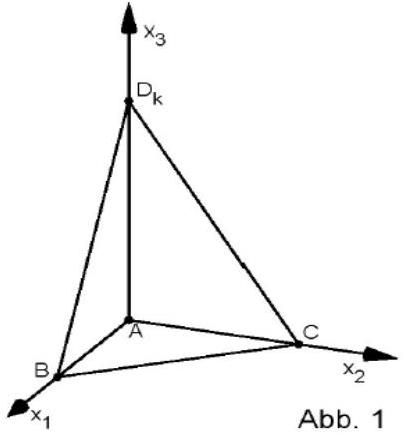
\includegraphics[max width=\textwidth, center]{2025_04_24_dd222e08aeda8e28cc23g-2(1)}\\
a) Begründen Sie, dass das Dreieck $B C D_{k}$ gleichschenklig ist.

Der Mittelpunkt der Strecke BC ist $\mathrm{M}(2|2| 0)$.\\
$\left|\overrightarrow{M D_{k}}\right|=\left|\left(\begin{array}{c}-2 \\ -2 \\ k\end{array}\right)\right|$ ist die Länge einer Höhe des Dreiecks $B C D_{k}$.\\
Bestimmen Sie den Flächeninhalt des Dreiecks $B C D_{k}$.\\
(1 VP)

Für jeden Wert von $k$ liegt die Seitenfläche $B C D_{k}$ in der Ebene $\mathrm{L}_{\mathrm{k}}: \mathrm{kx}_{1}+\mathrm{kx}_{2}+4 \mathrm{x}_{3}=4 \mathrm{k}$.\\
b) Ermitteln Sie denjenigen Wert von k, für den Größe des Winkels, unter dem die $x_{3}$-Achse die Ebene $L_{k}$ schneidet, $30^{\circ}$ beträgt.\\
(2,5 VP)\\
c) Zusätzlich zu den Pyramiden wird der in der Abbildung 2 gezeigte Quader betrachtet. Die Punkte A und Q(1|1|3) sind Eckpunkte des Quaders, die Seitenfläche des Quaders sind parallel zu den Koordinatenebenen. Für k= 6 enthält die Seitenfläche $B C D_{k}$ der Pyramide den Eckpunkt Q des Quaders. Für kleinere Werte von k schneidet die Seitenfläche $B C D_{k}$ den Quader in einem Vieleck. Für einen Wert von $k$ verläuft die Seitenfläche $B C D_{k}$ durch die Eckpunkte $P$ und R des Quaders.\\
Bestimmen Sie diesen Wert von k. (1,5 VP)\\
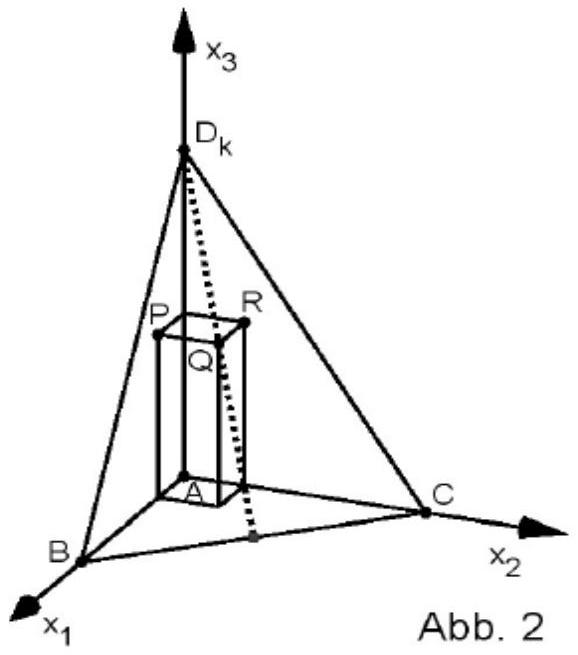
\includegraphics[max width=\textwidth]{2025_04_24_dd222e08aeda8e28cc23g-2} (Teilergebnis: $\mathrm{k}=4$ )\\
Geben Sie in Abhängigkeit von $k$ die Anzahl der Eckpunkte des Vielecks an, in dem die Seitenfläche $B C D_{k}$ den Quader schneidet.\\
d) Nun wird die Pyramide $A B C D_{6}$, d.h. diejenige für $\mathrm{k}=6$, betrachtet. Dieser Pyramide werden Quader einbeschrieben (vgl. Abbildung 3). Die Grundflächen der Quader liegen in der $\mathrm{x}_{1} \mathrm{x}_{2}$-Ebene, haben den Eckpunkt $A$ gemeinsam und sind quadratisch. Die Höhe h der Quader durchläuft alle reellen Werte mit $0<h<6$. Für jeden Wert von $h$ liegt der Eckpunkt $Q_{h}$ in der Seitenfläche $\mathrm{BCD}_{6}$ der Pyramide. Ermitteln Sie die Koordinaten des Punkts $Q_{h}$.\\
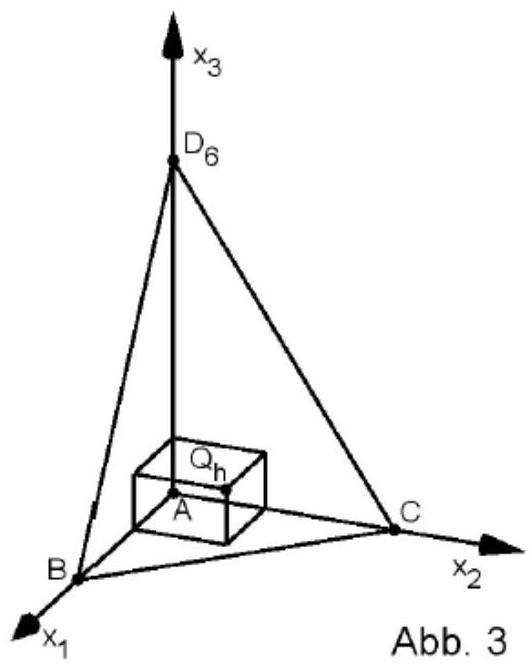
\includegraphics[max width=\textwidth, center]{2025_04_24_dd222e08aeda8e28cc23g-3}\\
(2 VP)

\section*{Lösungen}
\section*{Aufgabe B1}
a) Begründen Sie, dass das Dreieck $B C D_{k}$ gleichschenklig ist.

Berechnung der Seitenlängen des Dreiecks:

$$
\begin{aligned}
& |\overrightarrow{\mathrm{BD}}|=\left|\left(\begin{array}{c}
-4 \\
0 \\
\mathrm{k}
\end{array}\right)\right|=\sqrt{16+\mathrm{k}^{2}} \quad\left|\overrightarrow{\mathrm{CD}_{\mathrm{k}}}\right|=\left|\left(\begin{array}{c}
0 \\
-4 \\
\mathrm{k}
\end{array}\right)\right|=\sqrt{16+\mathrm{k}^{2}} \\
& |\overrightarrow{\mathrm{BC}}|=\left|\left(\begin{array}{c}
-4 \\
4 \\
0
\end{array}\right)\right|=\sqrt{16+16}=\sqrt{32}
\end{aligned}
$$

$\mathrm{Da}\left|\overrightarrow{\mathrm{BD}} \mathrm{K}_{\mathrm{k}}\right|=\left|\overrightarrow{\mathrm{CD}_{\mathrm{k}}}\right|$ gilt, ist das Dreieck gleichschenklig.\\
Bestimmen Sie den Flächeninhalt des Dreiecks $B C D_{k}$.\\
$\mathrm{A}=\frac{1}{2} \cdot|\overrightarrow{\mathrm{BC}}| \cdot\left|\overrightarrow{\mathrm{MD}_{\mathrm{k}}}\right|=\frac{1}{2} \sqrt{32} \cdot \sqrt{4+4+\mathrm{k}^{2}}=\frac{1}{2} \sqrt{32} \cdot \sqrt{8+\mathrm{k}^{2}}$\\
b) Ermitteln Sie denjenigen Wert von $k$, für den Größe des Winkels, unter dem die $\mathrm{x}_{3}$-Achse die Ebene $\mathrm{L}_{\mathrm{k}}$ schneidet, $30^{\circ}$ beträgt.

Schnittwinkelformel zwischen Gerade und Ebene: $\sin (\alpha)=\frac{|\overrightarrow{\mathrm{u}} \cdot \vec{n}|}{|\overrightarrow{\mathrm{u}}| \cdot|\overrightarrow{\mathrm{n}}|}$ Normalenvektor der Ebene: $\vec{n}=\left(\begin{array}{l}k \\ k \\ 4\end{array}\right) \quad$ Richtungsvektor der $x_{3}$-Achse: $\vec{u}=\left(\begin{array}{l}0 \\ 0 \\ 1\end{array}\right)$

$$
\begin{aligned}
\sin \left(30^{\circ}\right)=\frac{\left(\begin{array}{l}
0 \\
0 \\
1
\end{array}\right) \cdot\left(\begin{array}{l}
k \\
k \\
4
\end{array}\right)}{\sqrt{1} \cdot \sqrt{k^{2}+k^{2}+16}} & \left.\Leftrightarrow \frac{1}{2}=\frac{4}{\sqrt{2 k^{2}+16}} \right\rvert\, \cdot 2 \cdot \sqrt{2 k^{2}+16} \\
& \Leftrightarrow \sqrt{2 k^{2}+16}=8 \quad \mid \text { quadrieren } \\
& \Rightarrow 2 k^{2}+16=64 \\
& \Rightarrow k= \pm \sqrt{24}
\end{aligned}
$$

Wegen $\mathrm{k}>0$ gilt $\mathrm{k}=\sqrt{24}$.\\
c) Für einen Wert von $k$ verläuft die Seitenfläche $B C D_{k}$ durch die Eckpunkte $P$ und $R$ des Quaders. Bestimmen Sie diesen Wert von $k$.

Anhand der Koordinaten von $\mathrm{Q}(1|1| 3)$ können die Koordinaten von P bestimmt werden, der in der $\mathrm{x}_{1}-\mathrm{x}_{3}$-Ebene liegt: $\mathrm{P}(1|0| 3)$

Einsetzen von $P$ in die Ebenengleichung $L_{k}$ :\\
$\mathrm{k} \cdot 1+\mathrm{k} \cdot 0+4 \cdot 3=4 \mathrm{k}$\\
$\Leftrightarrow 3 k=12 \Leftrightarrow k=4$

Geben Sie in Abhängigkeit von k die Anzahl der Eckpunkte des Vielecks an, in dem die Seitenfläche $\mathrm{BCD}_{\mathrm{k}}$ den Quader schneidet.

Ebene für $\mathrm{k}=2$ : Schnittfläche ist ein Viereck\\
Dies gilt für alle Werte von k mit $0<\mathrm{k} \leq 3$.\\

Ebene für $\mathrm{k}=3,5$ : Schnitffläche ist ein Fünfeck.\\
Dies gilt für alle Werte von $k$ mit $3<k<4$.\\

Ebene für $\mathrm{k}=4$ und $\mathrm{k}=5$ : Schnittfläche ist ein Dreieck\\
Dies gilt für alle Werte von $k$ mit $4 \leq k<6$.\\
d) Ermitteln Sie die Koordinaten des Punkts $Q_{h}$.

Da der Quader eine quadratische Grundfläche hat, sind die $x_{1}$ - und $x_{2}$-Koordinaten des Punktes $Q_{h}$ identisch.\\
Allgemeine Koordinaten: $\mathrm{Q}_{\mathrm{h}}(\mathrm{u}|\mathrm{u}| \mathrm{h})$\\
Einsetzen in die Gleichung der Ebene $L_{6}: 6 x_{1}+6 x_{2}+4 x_{3}=24$\\
$6 u+6 u+4 h=24$\\
$\Leftrightarrow 12 u=24-4 h$\\
$\Leftrightarrow u=2-\frac{1}{3} h$\\
Die gesuchten Koordinaten lauten $Q_{h}\left(2-\frac{1}{3} h\left|2-\frac{1}{3} h\right| h\right)$


\end{document}